\chapter{Tecniche di giunzione}\label{chp:Giunzione}
Prevede di unire più componenti meccanici ne caso in cui non sia possibili ottenere un prodotto finito solo tramite le lavorazioni convenzionali e non convenzionali.
Le principali tecniche sono:
\begin{description}
\item[Fissaggio meccanico]: si tratta di fissaggi non removibili, quindi niente bulloneria piuttosto rivettature.
\item[Saldatura a freddo] Creazione di un legame metallurgico mediante adesione e diffusione.
Viene anche detta saldatura a freddo.
\item[Saldatura a caldo] Unione tramite fusione con l'uso di varie fonti di calore. Detta saldatura a caldo
\item[Brasatura] legami con l'aggiunta di metalli bassofondenti.
\end{description}

La giunzione viene utilizzata perché non siamo in grado di realizzare un prodotto complessivo in un unico colpo ma in successivi assemblaggi.
In genere si parla di giunzioni su metalli, non sono da escludere tecniche su ceramici e polimerici.

\section{Classificazione delle tecniche}
Le principali tecniche di fissaggio sono quelle della figura \ref{fig:Fissaggi}.

\begin{figure}
\centering
\subfloat[][\emph{Principali tecniche di fissaggio}\label{fig:Fissaggi}]
{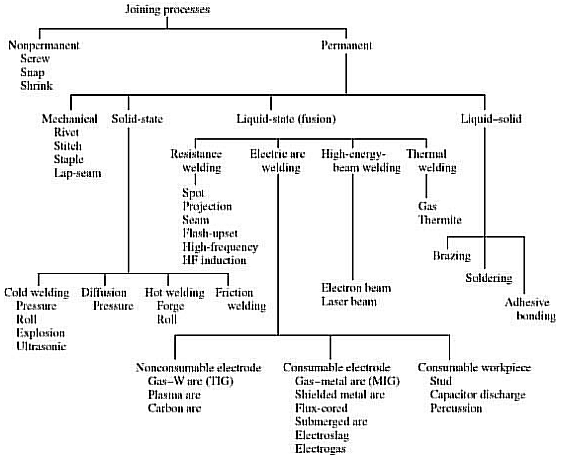
\includegraphics[width = \textwidth]{Fissaggi}}\\
\subfloat[][\emph{Confronto tra le tecniche di fissaggio}\label{fig:ConfFissaggi}]
{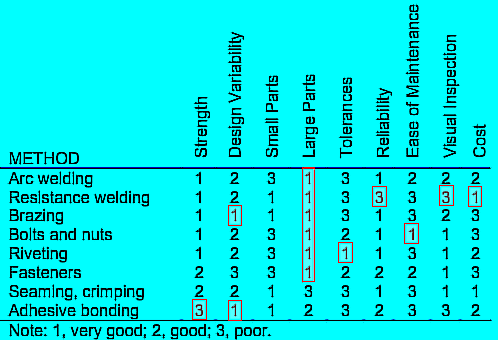
\includegraphics[width = 0.8\textwidth]{ConfFissaggi}}
\caption{Fissaggi}
\label{fig:TipiFissagi}
\end{figure}

Le tecniche di giunzione sono tra le tecniche che maggiormente si tende ad automatizzare.
In genere perché:
\begin{enumerate}
\item Il personale deve essere altamente formato.
\item In particolare per le saldature a caldo possono generarsi dei fumi nocivi o comunque ambienti pericolosi.
\end{enumerate}

\begin{description}
\item[\eng{arc welding}] Si sfrutta un arco elettrico per portare il materiale apportato a fusione.
\item[\eng{Resistence Welding}] la modalità non è diversa dalla precedente ma si sfrutta la legge di Ohm per scaldare il materiale.
\item[Brasatura] Si apporta del materiale bassofondente per legare i componenti.
\item[Bullonatura] Si sfruttano dei componenti meccanici per mantenere uniti più pezzi.
\item[Ritevettatura] Come prima ma non removibile
\item[Grafettatura] Si usano delle graffette per mantenere uniti più componenti.
\item[Aggraffatura] Specifico per lamiere, prevede di utilizzare delle specifiche forme per unire le lamiere, se ne era già parlato quando si è parlato nella piegatura delle lamiere al capitolo \ref{chp:Lamiere} a pagina \pageref{chp:Lamiere}.
\item[Incollaggio] Si utilizza un collante per tenere uniti più pezzi.
\end{description}

\section{Giunzioni meccaniche}
\subsection{Rivettatura}
Si tratta di una giunzione realizzata tramite una specie di chiodo che poi viene opportunamente lavorato per permettergli di mantenere giuntate le componenti, tramite la realizzazione di due teste aderenti ai componenti.
Si chiamano rivetti e alcuni sono mostrati in figura \ref{fig:TipiRivetti}.

\begin{wrapfloat}{figure}{O}{0pt}
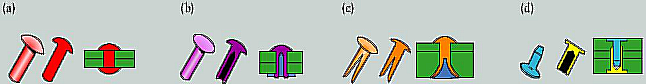
\includegraphics[width = \textwidth, angle = 90]{TipiRivetti}
\caption{Tipologie di rivetti}
\label{fig:TipiRivetti}
\end{wrapfloat}

La più comune tra le rivettature è a \textbf{Rivetti ciechi} come quelli in figura \ref{fig:RivettoCieco}.

\begin{figure}
\centering
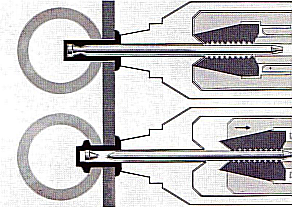
\includegraphics[width = 0.5\textwidth]{RivettoCieco}
\caption{Rivettatura cieca}
\label{fig:RivettoCieco}
\end{figure}

Il fatto che la rivettatura sia costosa rispetto ad altre giunzioni per il fatto che i componenti da giuntare devono già essere forati. Per cui si deve aggiungere una lavorazione aggiuntiva per poter rivettare.
In più la foratura è una fonte di incertezza sul comportamento a fatica del prodotto rivettato.
In più c'è il problema di dover sbavare i fori, in quanto le bave sono fonte di tensioni residue.

\begin{figure}
\centering
\subfloat[][\emph{Rivetto troppo lungo}\label{fig:TooLong}]
{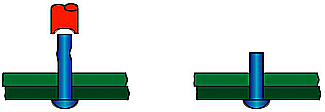
\includegraphics[width = 0.4\textwidth]{TooLong}}\quad
\subfloat[][\emph{Rivetto coperto}\label{fig:Covered}]
{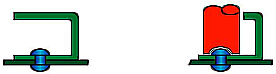
\includegraphics[width = 0.4\textwidth]{Covered}}\\
\subfloat[][\emph{Adesione non completa}\label{fig:NotProperly}]
{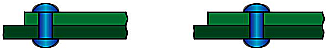
\includegraphics[width = 0.4\textwidth]{NotProperly}}\quad
\subfloat[][\emph{Troppo vicino al bordo}\label{fig:NearEdge}]
{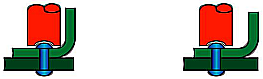
\includegraphics[width = 0.4\textwidth]{NearEdge}}
\caption{Considerazione sulla corretta rivettatura}
\label{fig:ConsRiv}
\end{figure}
I casi che possono portare alla rivettatura a fallire prematuramente possono essere:
scegliere correttamente la dimensione del rivetto perché si rischia di piegare il gambo piuttosto di realizzare la testa, caso \ref{fig:TooLong}.
Bisogna lasciare il giusto spazio affinché la macchina che crea la testa possa lavorare correttamente, caso \ref{fig:Covered}.
Anche il fatto di forare vicino ai bordi può essere fonte di pessimo comportamento a fatica, caso \ref{fig:NearEdge}.

\subsection{Grafettatura}
Si possono realizzare giunzioni tramite una graffetta per lamiere, \ref{fig:Graffettatura}.
Non hanno alti carichi di giunzione ma vengono alle volte usate per la realizzazione di mobili.

\begin{figure}
\centering
\subfloat[][\emph{Esempi di graffettatura}\label{fig:Graffettatura}]
{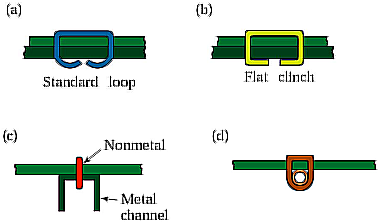
\includegraphics[width = 0.4\textwidth]{Graffettatura}}\:
\subfloat[][\emph{Realizzazione dell'aggraffatura}\label{fig:Aggraffatura}]
{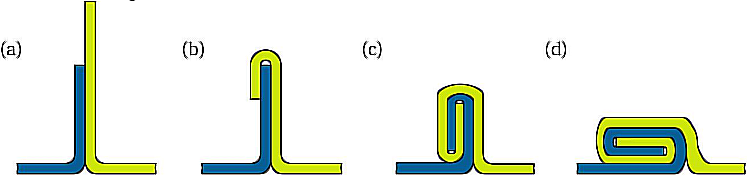
\includegraphics[width = 0.4\textwidth]{Aggraffatura}}\\
\subfloat[][\emph{Esempio di fissaggio \eng{snap-fit}}\label{fig:SnapFit}]
{\includegraphics[width = 0.4\textwidth]{Snapfit}}
\caption{Fissaggi meccanici di graffettatura, aggraffatura e \eng{snap-fit}}
\label{fig:GripMec}
\end{figure}

\subsection{Aggraffatura}
Si era anticipato l'argomento al capitolo \ref{chp:Lamiere} a pagina \pageref{chp:Lamiere}.
Comunque in figura \ref{fig:Aggraffatura} è riproposto il processo per realizzare tale tipo di giunzione.

\subsection{Giunzione a deformazione plastica}
Si realizzano delle piccole deformazioni del materiale per poter alloggiare delle giunzione tra un nucleo e manicotto.
Si possono sfruttare le variazioni dimensionali tramite variazione termica per poter facilitare la giunzione.
È una tecnica particolarmente usata in ambito elettrotecnico per realizzare gli ancoraggi ai morsetti ed eventuali collegamenti tra metalli diversi (tipo rame-alluminio).
Alcuni esempi sono alla figura \ref{fig:DefPlastGrip}.

\begin{figure}
\centering
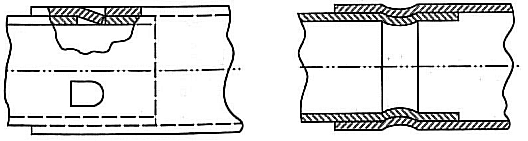
\includegraphics[width = 0.5\textwidth]{DefPlastGrip}
\caption{Alcuni esempi di fissaggio per deformazione plastica}
\label{fig:DefPlastGrip}
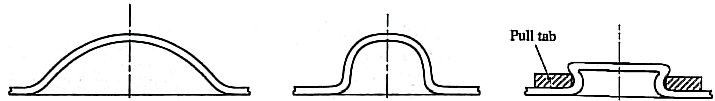
\includegraphics[width = 0.5\textwidth]{Ribattitura}
\caption{Processo di ribattitura}
\label{fig:Ribattitura}
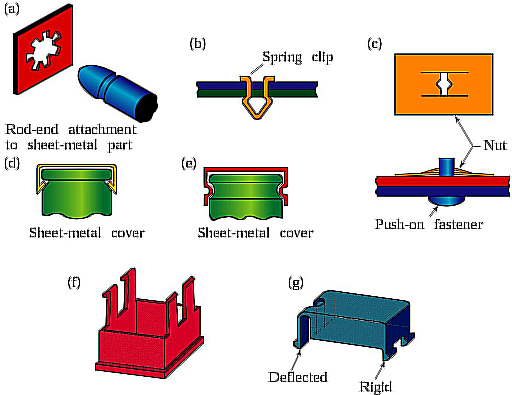
\includegraphics[width = 0.5\textwidth]{AltriGripMec}
\caption{Ulteriori metodi di fissaggio meccanico utilizzati}
\label{fig:AltriGripMec}
\end{figure}

\subsubsection{\eng{Sanp-fit}}
Detta anche chiusura a scatto, \ref{fig:SnapFit}. Viene molto apprezzata per:
\begin{itemize}
\item Basse forze di montaggio,
\item elevate forze di smontaggio,
\item semplici movimenti di montaggio,
\item \eng{feedback} sonoro o tattile,
\item facilità di automazione,
\item assenza di minuteria,
\item omogeneità dei materiali.
\end{itemize}

\subsubsection{Ribattitura}
Si "gonfiano" le lamiere e successivamente viene deformata per poter fissare entrambe tramite la deformazione di entrambe. 
Il processo è riportato alla figura \ref{fig:Ribattitura}.
Viene usata per la realizzazione dell'accoppiamento tra lattina e aprilattina.

Invece, alla figura \ref{fig:AltriGripMec} sono riportati ulteriori metodi di fissaggio meccanico.

\pagebreak


\section{Saldature allo stato solido}

\begin{figure}
\centering
\subfloat[][\emph{Ramo delle lavorazioni allo stato solido}\label{fig:SolidState}]
{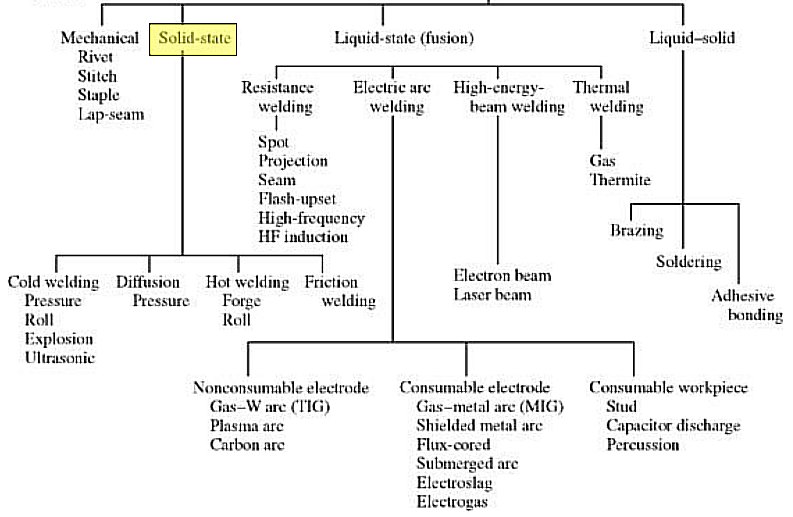
\includegraphics[width = 0.4\textwidth]{SolidState}}\quad
\subfloat[][\emph{Saldature a freddo}\label{fig:ColdWelding}]
{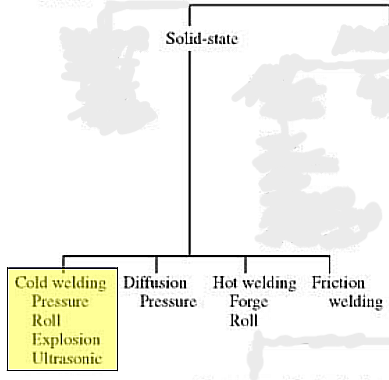
\includegraphics[width = 0.4\textwidth]{ColdWelding}}
\caption{Saldature allo stato solido col dettaglio delle lavorazioni a freddo}
\label{fig:SSCW}
\end{figure}

Le principali tecniche per giunzione allo stato solido vengono eseguite su:
\begin{itemize}
\item di testa,
\item ad angolo,
\item per sovrapposizione,
\item a spigolo
\end{itemize}
Mentre le principali tecniche sono quelle della figura \ref{fig:SolidState}.

Vengono realizzate senza portare a fusione il materiale.
La saldatura a freddo svincola dalla necessità di avere dei materiali che hanno temperature di fusione vicine.
Si prenda come esempio il caso di giuntare dei profili di rame con quelli di alluminio per la realizzazione di trasformatori elettrici.

Nella saldatura a freddo non si scalda il materiale, per cui è necessario avere un'ottima preparazione della superficie.
In particolare è opportuno che il substrato di entrambi i materiali debba esser preparato per poter eseguire correttamente la giunzione.
Deve venire a contatto senza che vi sia presenza di ossidi, polveri, impurezze, ecc\dots
Per rimuovere i contaminanti si possono pulire tramite solventi per rimuovere le impurità. Anche spazzolare contribuisce ad aumentare la rugosità superficiale con conseguente aumento dell'estensione della superficie del substrato, cioè l'area su cui realizzare il legame.
Poi si usa il moto relativo, che aiuta a rimuovere eventuali film di ossido e avvia il processo di fusione.
Con una successiva deformazione plastica si apre il film ossido portando alla luce il substrato duttile.
In teoria non sarebbe necessaria alcuna pressione per effettuare questo tipo di saldature. 
Viene comunque usata per deformare plasticamente i materiali, facendo in modo che le superfici si conformino l'una all'altra.
Favorendo la reciproca saldatura tramite l'ottenimento di un impasto  dei due materiali.

Per queste saldature il calore serve per favorire la duttilità dei materiali, facilitando l'intimo contatto dei due substrati.
Infatti, non è una necessità scaldare ma una conseguenza.

\subsection{Saldature a freddo}
Le possibilità della saldatura a freddo, come illustrato dal grafico \ref{fig:ColdWelding}, sono:
\begin{description}
\item[Saldatura a freddo per sovrapposizione]Si basa su una forte dilatazione delle superfici come illustrato alla figura \ref{fig:CWSovrap}.
\item[Saldatura a freddo di testa] generalmente usata per fili, si ha una forte pressione sulla testa dei componenti per poterli "impastare" dando deformazione alla superficie del substrato, ne è un esempio la seconda figura \ref{fig:CWSovrap}.
\item[Saldatura a freddo per laminazione] Con forti riduzioni di spessore della saldatura a rulli si ottiene una grande espansione della superficie. Il legame può essere impedito localmente con un distanziale.
Alla figura \ref{fig:CWRolling} viene presentato il metodo di funzionamento.
\item[Saldatura a freddo per esplosione] Si genera un'onda d'usto che provoca delle deformazioni all'interfaccia dei due materiali portandoli alla saldatura. Come si vede dalle figure \ref{fig:CWExplosive1} e \ref{fig:CWExplosive2}, si può operare in due maniere ottenendo la saldatura in entrambi i casi.
\item[Saldatura a freddo ad ultrasuoni] Si tratta di una lavorazione non convenzionale, anche se l'energia trasmessa è di tipo meccanico, grazie alle alte frequenze degli ultrasuoni si creano onde d'urto che portano anche in questo caso alla saldatura dei due materiali.
Vedi la figura \ref{fig:CWUltrasounds}. 
\end{description}


\begin{figure}
\centering
\subfloat[][\emph{Saldatura a freddo per sovrapposizione e di testa}\label{fig:CWSovrap}]
{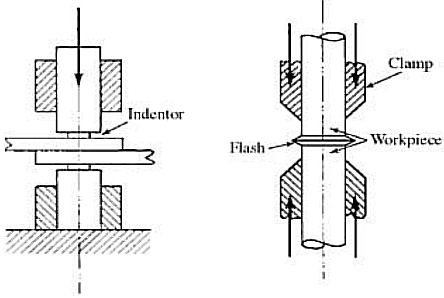
\includegraphics[width = 0.3\textwidth]{CWSovrap}}\quad
\subfloat[][\emph{Saldatura a freddo per laminazione}\label{fig:CWRolling}]
{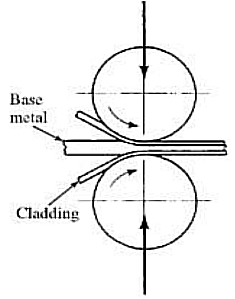
\includegraphics[width = 0.3\textwidth]{CWRolling}}\quad
\subfloat[][\emph{Saldatura a freddo con distanziali}\label{fig:CWDist}]
{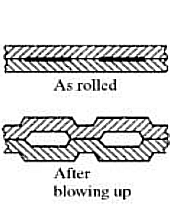
\includegraphics[width = 0.3\textwidth]{CWDist}}\\
\subfloat[][\emph{Saldatura a freddo per esplosione}\label{fig:CWExplosive1}]
{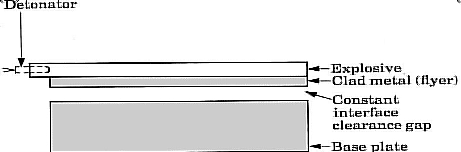
\includegraphics[width = 0.4\textwidth]{CWExplosive1}}\quad
\subfloat[][\emph{Ulteriore tecnica di saldatura a freddo per esplosione}\label{fig:CWExplosive2}]
{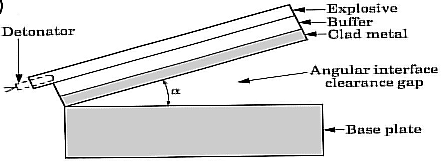
\includegraphics[width = 0.4\textwidth]{CWExplosive2}}\\
\subfloat[][\emph{Saldatura a freddo tramite ultrasuoni}\label{fig:CWUltrasounds}]
{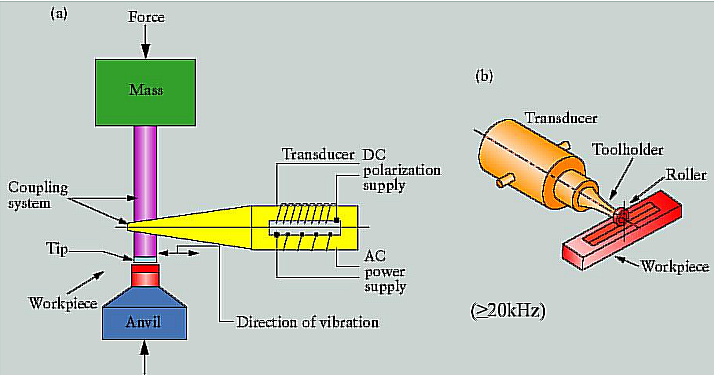
\includegraphics[width = \textwidth]{CWUltrasounds}}
\caption{Principali tecniche di saldatura a freddo}
\label{fig:CW}
\end{figure}

\subsection{Saldature per diffusione}
Si potrebbero eseguire anche senza avere temperature eccessivamente alte $\approx 0.5 T_m$. Nella pratica vengono comunque sfiorate le temperature normali per favorire la corretta avvenuta della giunzione.
Di fatto favorendo la diffusione degli atomi dei due materiali.
Tale tecnica si usa da secoli per realizzare oggetti placcati in oro.
Si era anticipato l'argomento quando si era accennato alla \textit{superplasticità}. Tale aiuta a unire la saldatura a freddo come le precedenti che la diffusione. Ciò realizza un giunto di altissima qualità.
Si raggiunge tale stato per poter deformare molto semplicemente e a ridotto impiego di forze, dei materiali che risulterebbero decisamente molto duri.
Anche la saldatura per diffusione è un processo molto lento.
Nella pratica, oltre alle alte temperature si preferisce porre un peso sopra alle zone da giuntare per ottenere una qualità migliore.
Tele tecnica permette di realizzare degli oggetti saldati alternativamente senza dover subire ulteriori lavorazioni. Ciò viene realizzato interponendo dei distanziali di nitruro di boro che impediscono la diffusione tra i due materiali, di fatto evitando la saldatura.

Si mette il tutto in un forno, si sovrappone al materiale una foglia d'oro e poi viene applicato un peso per garantire la diffusione.

\begin{figure}
\centering
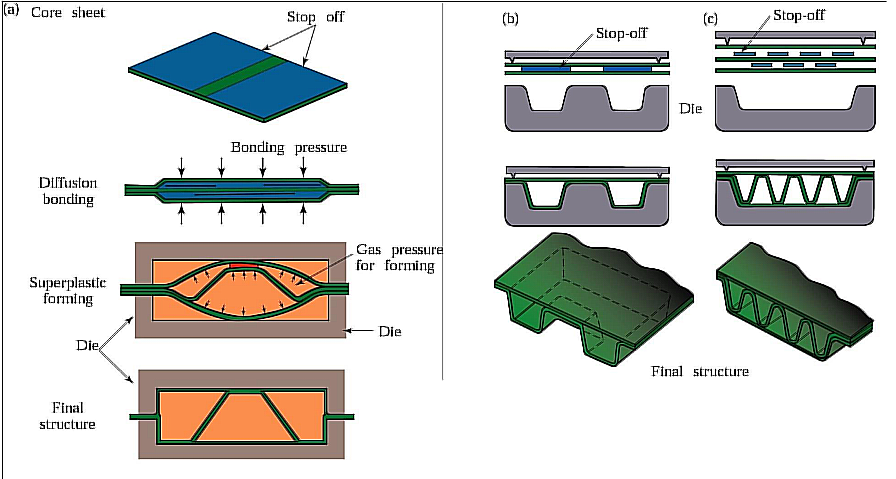
\includegraphics[width = \textwidth]{CWDiffusion}
\caption{Realizzazione per saldatura a diffusione di profili utilizzati in aeronautica}
\label{fig:CWDIffusion}
\end{figure}

Alla figura \ref{fig:CWDIffusion} viene presentato il processo produttivo di alcuni materiali generalmente utilizzati in ambito aeronautico. In genere si tratta di prodotti in lamiera che tramite questo processo è possibile produrli grazie a questa tecnica.
Si evita di utilizzare delle giunzioni rivettate che avrebbero un costo molto elevato, peso maggiore e tempo di produzione altrettanto elevato.

\subsection{Saldature a caldo}
Si rifanno direttamente alle lavorazioni per deformazione plastica a caldo già viste in precedenza.
Risulta essere la più antica forma di saldatura per materiali ferrosi.
C'è stata un'evoluzione nella tecnica di di tali la\todo{\\Aggiungi}

Fondamentalmente si può praticamente tutte le tecniche di riscaldamento, L'importante è la successiva pressione da dare ai materiali.
Con questo tipo di saldatura, in trazione si rompe il materiale base non il giunto.

\subsection{Saldatura a frizione}
Si tratta di una tecnica con cui scaldiamo gli elementi da giuntare.
\missingfigure{Saldatura per frizione}
L'attrito determina il riscaldamento dell'interfaccia in più la pressione simultanea andrà a giuntare i due pezzi. Si forma un colletto di bava
\missingfigure{Processo di saldatura per attrito}
Si presenta un piccolo errore nella figura perché si dovrebbe mettere in rotazione, premere poco.
Poi fermare la rotazione, aumentare la forza in cui si genera anche la bava. 
Per poi finire finché la zona pastosa non si raffredda.

\subsubsection{Friction Stir Welding}
Si tratta di una tecnica che si è sviluppata per la saldatura di teste per lamiere di spessore piuttosto pronunciato. 
Risulta interessante per via del fatto che la macchina necessaria per il raggiungimento dello scopo basta una fresa a controllo numerico.

L'utensile ruota, scalda il materiale delle due lamiere avvicinate, percorre un qualsiasi percorso di saldatura come se fosse una fresa. 

\section{Saldature a fusione}
Vengono definite come le uniche tecniche vere e proprie di fusione.
Si tratta delle tecniche di saldature più ampio ed utilizzato in ambito meccanico.

Si parla di saldatura eterogena se si apporta un terzo materiale per effettuare la saldatura, altrimenti omogenea.

Le principali categorie di saldatura sono:
\begin{description}
\item[Saldatura a resistenza]
\item[Saldatura arco elettrico]
\item[\dots]\todo{\\aggiungere}
\end{description}

Le velocità di raffreddamento sono alte, superiori a quelle della fonderia in stampo permanente. Dunque si possono ottenere delle zone che restano amorfe, oppure si hanno degli effetti di ingrossamento del grano per via del ciclo termico imposto tramite la saldatura.
Il grado di disomogeneità cresce passando dai metalli puri alle leghe multi fase e dipende anche dalla concentrazione di energia.

Un'aspetto importante durante una saldatura è \textbf{l'intensità di energia}: ovvero un parametro energia/area.
Con un'elevata intensità di energia si ottiene una saldatura profonda. Avendo una zona termicamente alterata è particolarmente stretta: per via del calore che ha meno tempo di diffondersi.
Inoltre, si hanno minori cambiamenti nella struttura metallurgica e minori sollecitazioni sul cordone di saldatura durante il raffreddamento.
Si riscontra anche una maggiore produttività.
Riuscire ad avere un'elevata intensità di energia ha parecchi benefit in termini di riuscita della saldatura.
\missingfigure{cordone saldatura profondo}
Al contrario si ha un cordone di saldatura particolarmente fino e disteso
\missingfigure{cordone di saldatura fino}

Considerando dei materiali monofasici: si suppone di giuntare due lembi dello stesso metallo puro con stesso materiale d'apporto.
In parte fondono anche i lembi.
Il materiale base adiacente alla zona fusa cambia proprietà.
\missingfigure{Caratteristica saldatura}
Se il materiale era incrudito c'è il rischio di ricristallizzazione e la dimensione dei grani e la dimensione dei grani cresce con la permanenza ad alta temperatura.
Se il materiale era ricotto i grani crescono di dimensioni.
In ogni caso ci sono grani grandi al bordo della zona fusa.
\missingfigure{Dimensione intergranulare nella ZTA}
La pozza di saldatura: ovvero dove si concentra la maggior parte dell'intensità di energia avrà una ben specifica forma.
In generale se si avesse solo un punto di saldatura questo avrebbe una pozza di forma circolare.
Aumentando la velocità di traslazione della fonte di energia si avrà una forma della pozza prima ellittica e poi maggiormente allungata all'aumentare della velocità.

Altri parametri che permettono di stimare la velocità di saldatura sono:
\begin{itemize}
\item Spessore del materiale
\item Conduttività del materiale
\item Temperatura e tempo di fusione
\item Calore latente del materiale
\end{itemize}

\subsection{Caratteristiche del giunto}
Passando da due materiali monofasici a delle leghe.
In corrispondenza del conrdone di saldatura si avranno delle dendriti colonnari particolarmente lunghe e fine per via dell'alta velocitùà di raffreddamento.
Tra la temperatura di Liquidus ($T_L$) e quella di Solidus ($T_S$)si ha una zona pastosa.
Elementi basso fondenti segregano ai bordi della zona fusa.

Oltre alle leghe, altra situazione comune è quella dei sistemi a più fasi.
I materiali a composizione eutettica non danno particolari problemi. L'unico punto cui fare attenzione è quella della formazione di strutture lamellari particolarmente fragili.
I problemi durante la solidificazione si presentano soprattutto nella \ac{ZTA}.
Infatti, nello specifico degli acciai, la diversa velocità di raffreddamento da delle trasformazioni formando martensite e per temperature più basse la bainite.
La martensite è particolarmente problematica perché oltre alla fragilità da dei problemi di tensioni residue nella \ac{ZTA}.
Per quanto riguarda la trasformazione delle fasi: l'eventuale materiale d'apporto si è supposto che avesse la stessa composizione del materiale base. IN generale questo non è vero: il materiale d'apporto non è quasi mai lo stesso materiale, ciò per evitare che ci siano delle trasformazione di cricche e trasformazione di fasi.
Si evitano le cricche ma si complica di più lo studio del comportamento della saldatura. In più, non si ha un equilibrio per via del fatto che non si sta raffreddando omogeneamente.
Le soluzioni solide in genere non danno problemi.
Gli eutettici tendono ad essere fragili, ma hanno buone qualità quando le due fasi sono duttili.
Composti intermetallici sono da evitare per via della loro fragilità.
Se la differenza tra le temperature di fusione è alta allora si parla di brasatura.
Perciò si parla di saldatura quando le due temperature di fusione sono abbastanza vicine.

\missingfigure{Grafico intervalli di durezza}
Il grafi dimostra quanto una saldatura a caldo possa influenzare la durezza del materiale base. Perciò per le applicazioni critiche si cerca di evitare l'utilizzo delle saldature. Dunque, è un aspetto da tenere bene a mente durante il processo produttivo.

\subsection{Difetti e qualità della saldatura a fusione}
Nella realizzazione della saldatura a fusione possono verificarsi dei difetti.
Si farà riferimento ad una saldatura\todo{\\aggiungi}
\missingfigure{Confronto 3 saldature}
Quando l'apporto di calore è insufficiente: perché ci si muove troppo rapidamente o per altri motivi, si forma un \eng{underfill} per cui si formano dei riempimenti non completi di materiale d'apporto ed eventualmente delle mancanze di fusione per cui non si ha un mescolamento dei due materiali.
Altro caso è quello dell'\eng{Overfill}: si ha un eccesso di materiale d'apporto. Ciò è dovuto alla troppo bassa velocità di traslazione in confronto all'energia specifica donata al materiale.
\missingfigure{confronto altri errori}
Anche la posizione dove apportare il materiale è cruciale, infatti si possono avere delle mancanze locali di materiale: per cui la saldatura ha un risultato pessimo anche se eseguita a regola d'arte.
Come per le saldature a freddo, anche per queste giunzione è opportuno preparare correttamente i due materiali da saldare. Perciò è opportuno rimuovere, in varie forme, i contaminanti sugli strati superficiali sui materiali base.
le reazioni chimiche indesiderate sono evitate isolando la zona del fuso col vuoto, con un'atmosfera protettiva o con delle scorie che si formano in superficie al cordone di saldatura. Per tale scopo si aggiungono dei materiali che legano con le impurità e le portano in superficie.
Bisogna prestare attenzione alle scorie: sono materiali fragili e bisogna eliminarle nel caso in cui la saldatura vada eseguita in più passate.
I gas rilasciati o formati durante la saldatura possono portare a una porosità che indebolisce il giunto e aumenta le tensioni; particolarmente pericoloso è l'idrogeno: si trova nell'umidità dell'aria.
la fluidità del fuso permette alle scorie e ai gas di raggiungere la superficie, liberandole dal cordone.
Le segregazioni bassofondenti provocano la formazione di cricche in quanto vengono respinte durante la solidificazione delle dendriti.

Le strutture saldate dovrebbero essere progettate tenendo conto delle dilatazioni termiche imposte durante il riscaldamento per la saldatura.
Ricordando che il cordone di saldatura impone una distorsione una volta raffreddato, lasciando tensioni residue sul materiale. Peggiorando il comportamento a fatica del materiale.
Queste tensioni residue sono tanto maggiori quanto l'intervallo di solidificazione del materiale è ampio. 
In più questi fenomeni di tensioni residue favoriscono la corrosione per \textit{tensocorrosione}.
Dunque si cerca di saldare delle leghe che presentano intervallo di solidificazione particolarmente rastremato.

Un accorgimento per ridurre gli effetti peggiorativi della saldatura è il \textbf{preriscaldamento}.
Riduce l'energia necessaria per il completamento della saldatura.
Riduce la velocità di raffreddamento permettendo la saldatura di materiali in cui il raffreddamento rapido provoca la formazione di fasi fragili.
Aiuta ad allontanare l'idrogeno.
Riduce il ritiro differenziale, le distorsione e le tensioni residue.
inevitabilmente si ha una tendenza alla formazione di grani cristallini più grandi per via della temperatura.
altro beneficio è dato dalla \textbf{pallinatura}.
Imponendo delle tensioni di compressione sul materiale base si migliora il comportamento del materiale saldato.
In più, grazie alla pallinatura si possono rimuovere delle scorie presenti sula superficie del cordone precedente: utile per saldature successive.

Si può pensare di eseguire dei trattamenti termici post-saldatura: ad esempio una ricottura di distensione aiuta a rimuovere eventuali tensioni residue. Può portare a dei fenomeni di sovrainvecchiamento per le leghe che hanno indurimento per precipitazione.
Eventualmente anche la normalizzazione può avere degli effetti benefici.
Eventualmente trattamenti di tempre e simili permettono di gestire opportunamente il metallo dopo la saldatura.

\subsection{Intensità di energia}
L'intensità di energia è:
\begin{equation}
I_e = \frac{\overbrace{E_c}^{\text{Energia ceduta al sistema}}}{\underbrace{A}_{\text{Area di saldatura}}}
\end{equation}

\paragraph{Cannello ossiacetilenico} ha un'intensità di risaldamento di $1 \div 10 \unit{\W/\mm^2}$ particolarmente apprezzato perché non è richiesta l'alimentazione elettrica, per cui è possibile saldare anche in zone dove non arriva la rete elettrica.
\paragraph{Saldatura ad arco} $10 \div 1000 \unit{\W/\mm^2}$  
\paragraph{Fascio laser o elettronico} $1000 \div 10000 \unit{\W/\mm^2}$ ne risulta una saldatura di qualità molto alta. Vengono anche definite come saldature \eng{kayhole}.

Negli altri metodi di saldatura, il metodo di riscaldamento avviene tramite corrente elettrica. Perciò anche il sistema di controllo deve essere di buona qualità. Alcuni sistemi di saldatura elettronica prevedono dei sistemi di retroazione per ottenere un migliore risultato.

\section{La saldabilità}
\paragraph{Acciai ferritici} Sono materiali facilmente saldabili bisogna prestare attenzione all'eventuale formazione di martensite. Comportamento tipico per gli acciai altamente temprabili.
Il preriscaldamento e il post riscaldamento possono aiutare a migliorare la situazione.
\paragraph{Lamiere rivestite}
Nella saldatura a resistenza lo zinco evapora, crea un plasma e porta a polverizzazione e porosità.
Perciò lo zinco presenta una criticità nella saldatura di materiali zincati. Perciò il contenuto di zinco non deve essere eccessivo e la temperatura controllata.
\paragraph{Acciai inossidabili}
Le condizioni di saldatura devono essere scelte per impedire la formazione di $Cr_2O_3$ e carburi di cromo.
Negli austenitici la formazione degli ossidi di cromo ed eventuali carburi è ostacolata con varie tecniche.
Per evitare la formazione di ossidi e carburi vengono aggiunti degli elementi che formano dei carburi stabili.
\paragraph{Zinco} Ossida e vaporizza molto facilmente, percui è essenziale avere un accurato controllo della temperatura di saldatura.
\paragraph{Alluminio e magnesio} Entrambi sono facilmente saldabili ma in genere devono essere protetti tramite atmosfere a gas inerte data la facilità di entrambi ad ossidare. Entrambi sono caratterizzati dalla formazione di ampie tensioni residue, per cui è opportuno effettuare dei \ac{TT} dopo il processo di saldatura.
\paragraph{Leghe a base di rame} Il rame puro si ossida piuttosto bene se deossidato
\paragraph{Nichel} L'aspetto critico è lo zolfo perché se presente in percentuali bassissime infragilisce molto la struttura a base di nichel.
\paragraph{Leghe di titanio e refrattarie} Tanto più alta è la temperatura di fusione tanta è la facilità di creare ossidi: per cui si preferisce usare delle tecniche di saldatura ad alta intensità di energia.

\section{Saldatura a resistenza}
Si sfrutta l'effetto Joule per portare a fusione il materiale.
Per cui. I due materiali vengono premuti tra loro. Si applica per un certo numero di cicli una specifica intensità di corrente che andrà a riscaldare i due componenti.

Il problema principale è quella per cui la massima resistenza elettrica sia tra gli elementi da giuntare. Altrimenti si ha il massimo riscaldamento in altri punti del materiale che non sono coinvolti nella saldatura.
Perciò si esclude per tale tecnica la giunzione di leghe di rame e alluminio, essendo buoni conduttori non presenterebbero delle resistenze tali da generare effetto Joule interessante.

Infatti tale tecnica viene particolarmente usata per saldare le lamiere delle automobili.
\missingfigure{Saldatura a resistenza}
Le differenze di tensione sono piuttosto basse. Saranno le intensità di corrente ad essere decisamente alte. Ricordando che:
\begin{equation}
J = I^2Rt
\end{equation}
La massima resistenza elettrica \textbf{deve} essere tra le due lamiere.
Altrimenti si salderebbero gli elettrodi alle lamiere e non le due lamiere.
In generale gli elettrodi devono essere di materiale altamente conduttivo (rame, allumino) e spesso raffreddato per garantirne la durata.
L'affermazione di tale tecnica è data dal fatto che la pulizia superficiale è relativamente importante. Per selezionare i migliori parametri vengono spesso realizzate delle prove tecnologiche distruttive per valutare la riuscita della saldatura.

Questo tipo di saldatura non realizza un vero e proprio cordone di saldatura. In generale si realizzano dei punti di saldatura.
Per realizzare una specie di cordone si realizzano più punti di saldatura ravvicinati, garantendo anche la tenuta ai liquidi.
\missingfigure{Esempio Mini Minor}
\missingfigure{Processo di saldatura a resistenza}

\subsection{Saldatura su rilievo}
Si tratta di una tecnica utilizzata per controllare meglio il punto di saldatura. Per quanto riguarda il resto, non cambia nulla rispetto alla precedente.
\missingfigure{Saldatura su rilievo}
\todo[inline]{Le figure devono essere poste come sottofigure commentate}

\missingfigure{Saldatura a resistenza a rulli}
\todo[inline]{Aggiungere il commento alla saldatura a rulli}

\subsection{Saldatura a scintillio}
viene anche chiamata \eng{Flash Upset Weld}, si differenzia rispetto alle precedenti per:
\begin{itemize}
\item Geometria: questa è una saldatura di testa
\item Processo: la differenza di potenziale viene applicata prima che i due elementi vengono a contatto.
\item Il metallo fuso viene espulso
\end{itemize}

In questo caso il metallo fuso viene espulso.
La saldatura si forma ricalcando le superfici calde e solide.
Una buona saldatura verrà prodotta solo de la velocità di avvicinamento, corrente e tensione, corsa totale \todo{\\Completa}
\missingfigure{Esempio saldatura delle rotaie}

\section{Saldature ad arco}
L'arco si riferisce al fatto che la scintilla che si crea è prolungato nel tempo: una scintilla stabile.
Tale genera il calore che porta a fusione il materiale.
In generale ha un'ottima resistenza, sono adatte per componenti di grosse dimensioni e le tolleranze sono limitate.
Lo sviluppo delle tecniche si ha per sopperire a diversi aspetti negativi di tali saldature.

L'arco elettrico fornisce il calore per fondere il metallo, il polo collegato all'elettrodo negativo è detto catodo e sarà lui ad essere saldato all'altro elemento, infatti dal catodo partono gli elettroni per realizzare l'arco elettrico che di fatto diventa un plasma.
alle volte si sfruttano dei gas inerti per salvaguardare gli elettrodi.
Il flusso degli elettroni è responsabile de 85\% del trasferimento dell'energia. 

\missingfigure{Schema saldatura ad arco}

Risulta fondamentale il flusso di elettroni in quanto da quello si hanno diversi cordoni di saldatura.
Ad esempio con le lamiere sottili si usa invertire i due poli in quanto non si è interessati ad avere una saldatura profonda.

Nel caso di alluminio e magnesio si usa invertire la polarità per favorire lo strappo degli strati di ossido dai metalli.
Si può anche pensare di usare una corrente alternata per tale scopo.

Il calore prodotto è in parte disperso nell'ambiente circostante, soprattutto in presenza di correnti molto basse.

La protezione del cordone di saldatura si effettua tramite gas inerte oppure tramite la formazione di scorie che emergono dal cordone di saldatura, facendo in modo che le impurità salgano in superficie piuttosto di rimanere dentro il cordone.

L'elettrodo può essere permanente o consumabile.

Quindi delle suddivisione può essere fatta tra 4 parametri: Metodo di protezione: gas inerte o scorie; elettrodo consumabile o permanente.

\missingtable{Acronimi tipologie di saldatura ad arco}

vediamo ora le due tecniche di saldatura ad arco tramite elettrodo permanente.

\subsection{Saldatura ad arco con elettrodo permanente}
è detta saldatura \textbf{GTAW} o \textbf{TIG}.
Il materiale che fonde è il materiale base detta \textbf{saldatura autogena} oppure con materiale d'apporto.
Nella \texttt{GTAW} elettrodo e saldatura sono protetti da gas inerte.

In generale il catodo è l'elettrodo, soprattutto se di tungsteno, mentre si preferisce invertire la polarità quando il materiale base è alluminio o magnesio.

Per attivare l'arco: l'elettrodo viene allontanato a velocità controllata p si usa in arco ausiliario.
Una corrente ad alta frequenza aiuta l'attivazione e il mantenimento di tale arco.

In genere si ottengono delle saldature di alta qualità.
In più, la saldatura è visibile per successive ispezioni.

Bisogna prestare attenzione al mantenimento dell'elettrodo: non può surriscaldarsi e non deve entrare in contatto col pozzo di fuso.

\subsection{Saldatura ad arco al plasma}
In questo casso, a differenza della precedente, sia hanno 2 gas: uno di protezione della saldatura e l'altro che verrà ionizzato per realizzare il plasma.
Di solito si preferisce far passare il plasma attraverso un piccolo foro per garantire maggiore concentrazione del plasma.
Inizialmente il plasma non viene avviato tra elettrodo e il materiale base, bensì si attiva internamente alla \textbf{torcia}. Solo successivamente si avvia la corrente di saldatura che permetterà al plasma di concentrarsi sul materiale da saldare.

A bassa densità di corrente la zona fusa è simile a quella ottenuta nella saldatura ad arco convenzionale.
Ad alte densità di corrente prevale la modalità \eng{keyhole}.

\missingfigure{Tecnica di saldatura ad arco trasferito e non trasferito.}

Le due tecniche di saldatura al plasma sono
\begin{description}
\item[Ad arco non trasferito] in cui il plasma viene generato internamente alla torcia e resta all'interno della torcia. Sarà l'irraggiamento a scaldare il materiale.
\item[Ad arco trasferito] In questo caso si ha un classico arco di plasma in cui l'arco passa dalla torcia al prezzo, scaldandolo.
\end{description}

\missingfigure{Confronto tra saldature}

la saldatura al plasma si caratterizza per i valori particolarmente elevati di temperatura che si riescono a raggiungere. Ciò permette di lavorare molto più velocemente rispetto ad altre tecniche.

Orsa si vedranno le tecniche di saldatura con elettrodo consumabile.
In pratica l'elettrodo stesso diventa il materiale d'apporto.

\subsection{Saldatura ad arco con elettrodo consumabile}
L'elettrodo è un metallo conduttore che deve consumarsi per divenire il materiale d'apporto.
La tecnica si definisce come \textbf{GMAW} o \textbf{MIG}. 
Anche qui si sfrutta un gas protettivo.

L'elettrodo è collegato al terminale positivo e la densità di corrente determina la modalità di trasferimento del metallo.
Ciò si vuole perché è l'elettrodo che deve cedere degli ioni per depositarsi sul materiale base. In generale si trova un cordone di saldatura peggiore dei precedenti.

In questo caso non sono gli elettroni che danno la maggior parte dell'energia per scaldare il materiale. Bensì la densità di corrente.
In particolare, correnti a bassa densità, si ha un trasferimento per corto circuito, il gfas è scelto per minimizzare gli spruzzi perché il processo di saldatura è un susseguirsi di avvicinamento e allontanamento dell'elettrodo. Così al riscaldamento dell'elettrodo si scioglie una goccia.
A densità intermedia si ha un trasferimento globulare, sono possibili solo saldature su piani orizzontali.
Mentre a densità elevate si ha un deposito per spray ed è possibile saldare in qualsiasi direzione perché le gocce sono molto piccole e non risentono della gravità. Tra l'altro è la tecnica che dà la migliore finitura al cordone.
La corrente utilizzata è a impulsi.
Questa saldatura permette di saldare anche lunghe distanze per via del fatto che l'elettrodo è disponibile sul mercato in rocchetti.
in più il processo può essere automatizzato.

Un aspetto a cui prestare particolare attenzione è il fatto che queste tecniche vengono eseguite al chiuso. Ciò per evitare che venti possano spostare i gas protettivi lasciando scoperto il cordone di saldatura.

\subsection{Saldatura ad arco con elettrodo rivestito}
Si tratta di una tecnica \textbf{SMAW}. In questo caso l'elettrodo è ricoperto da un materiale protettivo che permetterà la formazione delle scorie.
Ciò è un problema perché tale tecnica è eseguita manualmente per il fatto che le bacchette hanno una lunghezza piuttosto limitata e spesso è necessario interrompere la lavorazione.
Come vantaggio il fatto che essendo il protettivo già sul fondente, non è necessario l'utilizzo di gas protettivi e può essere eseguita in ambienti aperti.

Se scelto in maniera ottimale, il protettivo dell'elettrodo, può migliorare la situazione in termini di saldatura.

Le bacchette sono realizzate in quel modo perché il protettivo è un materiale particolarmente fragile, per cui non sarebbe possibile realizzare supporti più lunghi.
Si tratta di una saldatura piuttosto lenta per via della sua natura.

In passato per a la tecnica più utilizzata in assoluto.

\subsection{Saldatura ad arco con fondente intubato}
Trattasi della tecnica \textbf{FCAW}.
Il vantaggio di avere il protettivo intubato è quello di avere una qualità migliore e più profondo. Il materiale d'apporto si presenta come piattina cava contenente il protettivo.

\missingfigure{Saldatura FCAW}

\subsection{Saldatura ad arco sommerso}
Indicata \textbf{SAW}.
Si tratta di una tecnica particolarmente utilizzata in campo automatico.
In questo caso non elettrodo e fondente non sono più inclusi in un unico corpo bensì sono organi separati.
Questa saldatura può essere usata solamente su superfici orizzontali.

\missingfigure{saldatura SAW}

\subsection{Saldatura ad arco con elettroscoria}
La sigla è \textbf{ESW}.
In questo caso la saldatura deve essere realizzata in verticale.
Si usa per produrre giunti di grosso spessore.
Il filo dell'elettrodo è all'interno di una pozza di scoria fusa.
L'arco viene spento dalla scoria e il calore è fornito dalla resistenza elettrica della scoria.
Pattini di rame trattengono fuso e scoria.

I pattini di rame raffreddati ad acqua chiudono lo spazio tra le parti da saldare per evitare che il fuso e la scoria fuoriescano.
La testa di saldatura viene sollevata mentre il deposito di saldatura si accumula.

\subsection{Saldatura ad arco a perno}
Sigla \textbf{SWP}.
In questo caso non si ha la necessità di un vero e prorprio materiale d'apporto, saranno i componenti da giuntare ad essere l'apporto.
Si tratta di una saldatura autogena.
Nella saldatura a perni l'arco elettrico è mantenuto tra la sporgenza di un pezzo e la superficie dell'altro.
Dopo fusione i 2 pezzo vengono schiacciati uno contro l'altro.
Un anello ceramico concentra l'argo, protegge dall'ossidazione e contiene il fuso.
Il diametro \todo{\\Aggiungi}

\missingfigure{SWP}

L'anello ceramico svolge varie funzioni:
\begin{itemize}
\item Concentra l'arco,
\item limita l'ossidazione 
\item Contiene il fuso.
\end{itemize}

\section{Automazione delle saldatura}
L'obbiettivo è quello di saldare il più possibile in maniera automatica.
Si per evitare l'impiego di operatori, sia per ottenere delle saldature a qualità migliori.
Il controllo del processo è sempre più spesso automatico. La forma degli impulsi elettrici è controllata da dispositivi elettronici.
I valori ottimali di corrente velocità di spostamento e velocità di avanzamento degli elettrodi vengono impostati e controllati tramite una macchina \ac{CNC}.
La cianfrinatura o viessol è una particolare lavorazione che serve a preparare i lembi prima che subiscano il
\todo[inline]{Da rivedere dalle slide}
\begin{itemize}
\item facilitare la \todo{\\aggiungi}
\end{itemize}

In alcuni casi viene eseguita in passate successive.
Si nota dalla figura \todo{\\Aggiungi ref} che le successive passate vìdovrebbero essere esguite alternativamente tra 

\section{Saldature chimiche}
\subsection{Saldatura con cannello ossiacetilenico}
Si usa l'acetilene perché il gas che fonde a temperatura più alta.
Però la temperatura massima che siraggiunge con questa tecnica, arriva fino a $3400\unit{\celsius}$. Si usa in ambito artigianale, per delle riparazione e, in particolare, per tutti quegli ambienti dove non è presente la corrente elettrica.

Per realizzare tale saldatura sono necessarie due bombole una con l'acetilene e l'altra con l'ossigeno.
La fiamma che si ottiene si divide in 3 zone ben definite.
\begin{enumerate}
\item Prima combustione nella zona interna, genera 1/3 del calore.
\todo{\\Aggiungi la reazione chimica}
\item I prodotti della reazione determinano la seconda zona riducente.
\todo{\\Aggiungi le formule chimiche}
\item Terza zona di combusione.
\end{enumerate}

Il fatto che la reazione sia riducente permette di utilizzare tale tecnica in particolare con gli acciai al carbonio.
La versatilità del controllo manuale, la possibilità di avere fiamma neutra, ossidante o riducente, la possibilità di \moretodo{\\aggiungi}

\missingfigure{Cannello e confronto qualità}

\missingfigure{Tipi di fiamme}

\subsection{Saldatura alla termite}
Si tratta di una tecnica che può sostituire la saldatura a resistenza tramite scintillio.
La termite è una miscela di un ossido metallico e un materiale puro.
\moretodo{\\integra con le slide}
Si tratta di una reazione di ossidoriduzione. per cui si ottiene un'ossidato che libera energia e ferro. Si possono aggiungere delle altre particelle di materiali per evitare di alzare troppo la temperatura del metallo.
Il ferro così ottenuto colerà verso il basso e salderà i componenti.

Si realizza uno stampo con una tramoggia in cui sarà presente la termite, durante la reazione colerà il ferro dentro lo stampo che poi dovrà essere distrutto e il pezzo andrà ripulito.

\moretodo[inline]{Aggiungere \textbf{Brasatura} e completare il capitolo}